\chapter{Implementation}

Databases store data persistently on a hard disk, and since most hard
disks in use today are revolving magnetic disks, databases are highly
optimized for this.

Revolving magnetic disks, as opposed to solid state disks, have a
physical disk that spins under a moving read/write head.  Such disks
are organized into sectors (a slice of the disk), and each sector is
further divided into blocks of a fixed number of bytes.  In order to
read to or write a block in a sector of the spinning disk, both the
disk and head must move, which is the bottleneck in the speed of a
drive.

Databases are optimized for this scenario, in that they minimize the
number of blocks to be read from the drive, thus minimizing the amount
of disk and head movement.

\section{B+ Trees}

The biggest optimization to minimize block retrievals is to store as
much information within a block as possible.  A B+ tree is a tree with
a large branching factor wherein all data nodes are leafs.

In a B+ tree, a branching factor $b$ is specified and largely
determines the structure of the tree.  The branching factor $b$ is an
upper bound on the number of children each internal node can have.

The data stored in a B+ tree must be associated with a fully ordered
key, which determines the order of the data in the leaf nodes.

\begin{center}
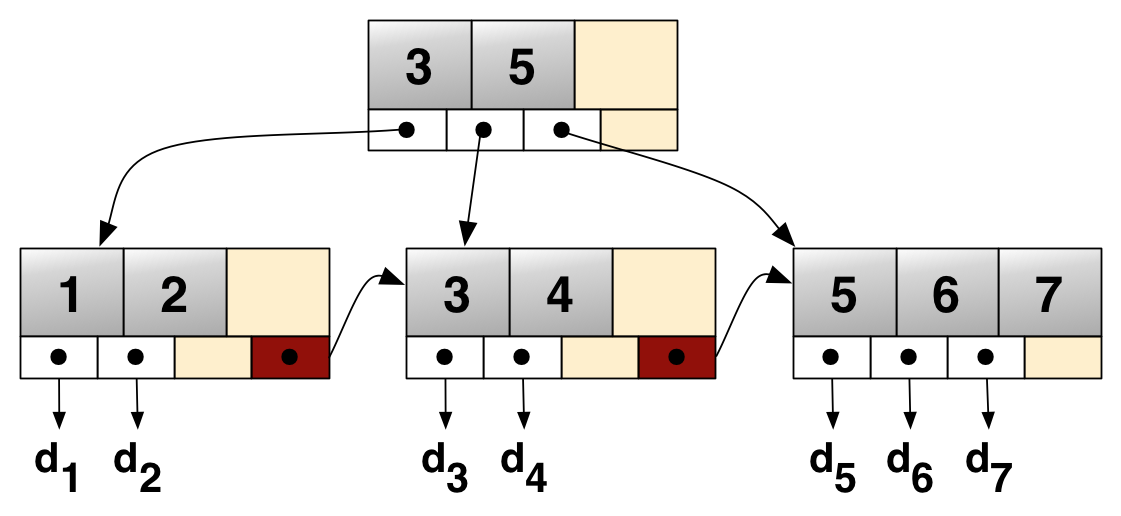
\includegraphics[scale=0.4]{figs/Bplustree.png}
\figcaption{A B+ tree, image courtesy of
  \href{https://en.wikipedia.org/wiki/File:Bplustree.png}{Wikipedia}}
\end{center}

A B+ tree has many types of nodes:

\begin{itemize}

\item A leaf node which contains data.

\item An internal root node which contains from 2 to $b$ references to
  internal nodes.  This node also stores the key values on which the
  internal nodes are split.

\item An internal (non-root) node which contains between $\lceil b/2
  \rceil$ references to either other internal or leaf nodes.  If this
  node points to internal nodes, it contains the keys on which the
  internal nodes are split.  If this node points to leaf nodes, it
  contains the keys of the leaf nodes it references.

\end{itemize}

The smallest possible B+ tree contains just a single leaf node
containing data.  

In general, when a datum $d$ is added to the tree, we find the
location where $d$ ought to be.  

If that location is in the root leaf node, and the root leaf node
contains less than $b$ data we simply add it and we're done.  If there
are $b$ other data on the root leaf node, it is split into 2 leaf
nodes referenced to by an internal root node.

If $d$ belongs in a non-root leaf node $N$, containing less than $b$
other data we can simply add $d$ and we're done.  If $N$ contains $b$
other data, we must split $N$ into two leaf nodes $N_1$ and $N_2$.  We
remove the reference to $N$ from $N$'s parent, and add the references
to $N_1$ and $N_2$.  Note that this may cause a cascade of node splits
up to the root.

The complexity of insertion is $\BigOh{log_b(n)}$.  Note that our choice
of $b$ usually depends on the block size of the disk.  We would like
each node to occupy an entire block on disk, which minimizes block
reads.
